\documentclass[12pt]{article}

\usepackage{amsmath}
\usepackage{amssymb}
\usepackage{graphicx}
\usepackage{color}
\usepackage[total={6in,8in}]{geometry}
\usepackage{amsthm}

\usepackage{enumitem}
\usepackage{centernot}

\newcommand{\N}{\mathbb{N}}
\newcommand{\Z}{\mathbb{Z}}
\newcommand{\Q}{\mathbb{Q}}
\newcommand{\R}{\mathbb{R}}
\newcommand{\C}{\mathbb{C}}
\newcommand{\sn}{\mathfrak{S}}
\newcommand{\ve}{\varepsilon}
\setlength{\parindent}{1cm}


\author{Marika Swanberg and Jillian James}
\title{Cache Optimization}
\date{}
\begin{document}
\maketitle
\section{Optimization}
Our data from last homework showed a sharp increase in the average response time as we increased the number of items in the cache. We hypothesized that this was due to how our FIFO eviction was implemented. As it was implemented previously, our FIFO was essentially $O(n)$. We decided that this would be the most important thing to optimize, so we focused our energy here. 

We had previously implemented FIFO by keeping track of the order in which the elements were added to the cache and subsequently evicted the oldest item by looping through all of the items. We replaced this method with a simple queue. Our \texttt{set()} method enqueues items and our \texttt{evictor()} method dequeues the item and deletes that item from the cache. This is an $O(1)$ algorithm that we essentially should have had this whole time.

\section{Results}
\bigskip 

\begin{center}
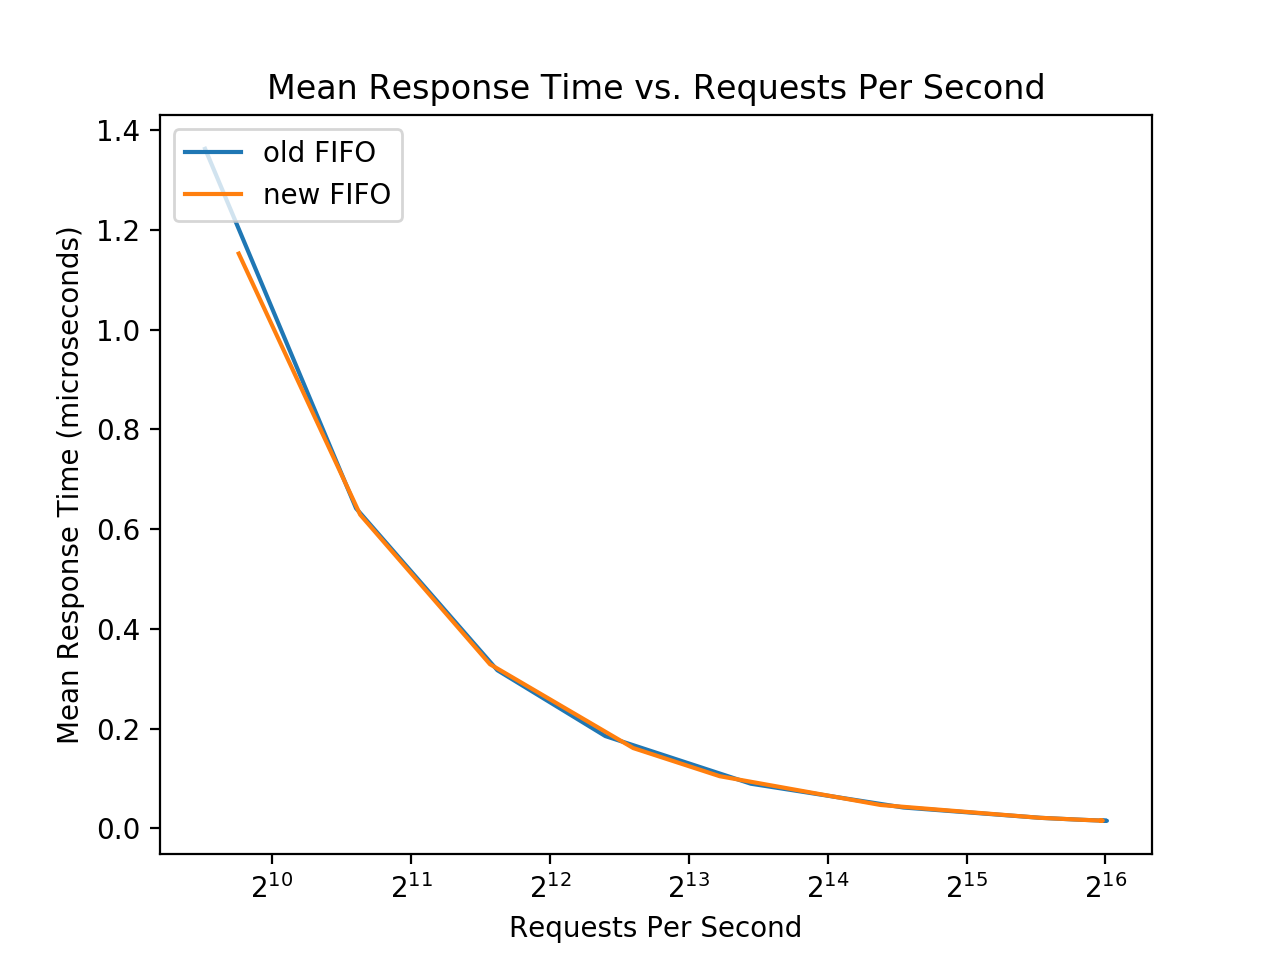
\includegraphics[scale=0.75]{reqs_per_sec_newold.png}
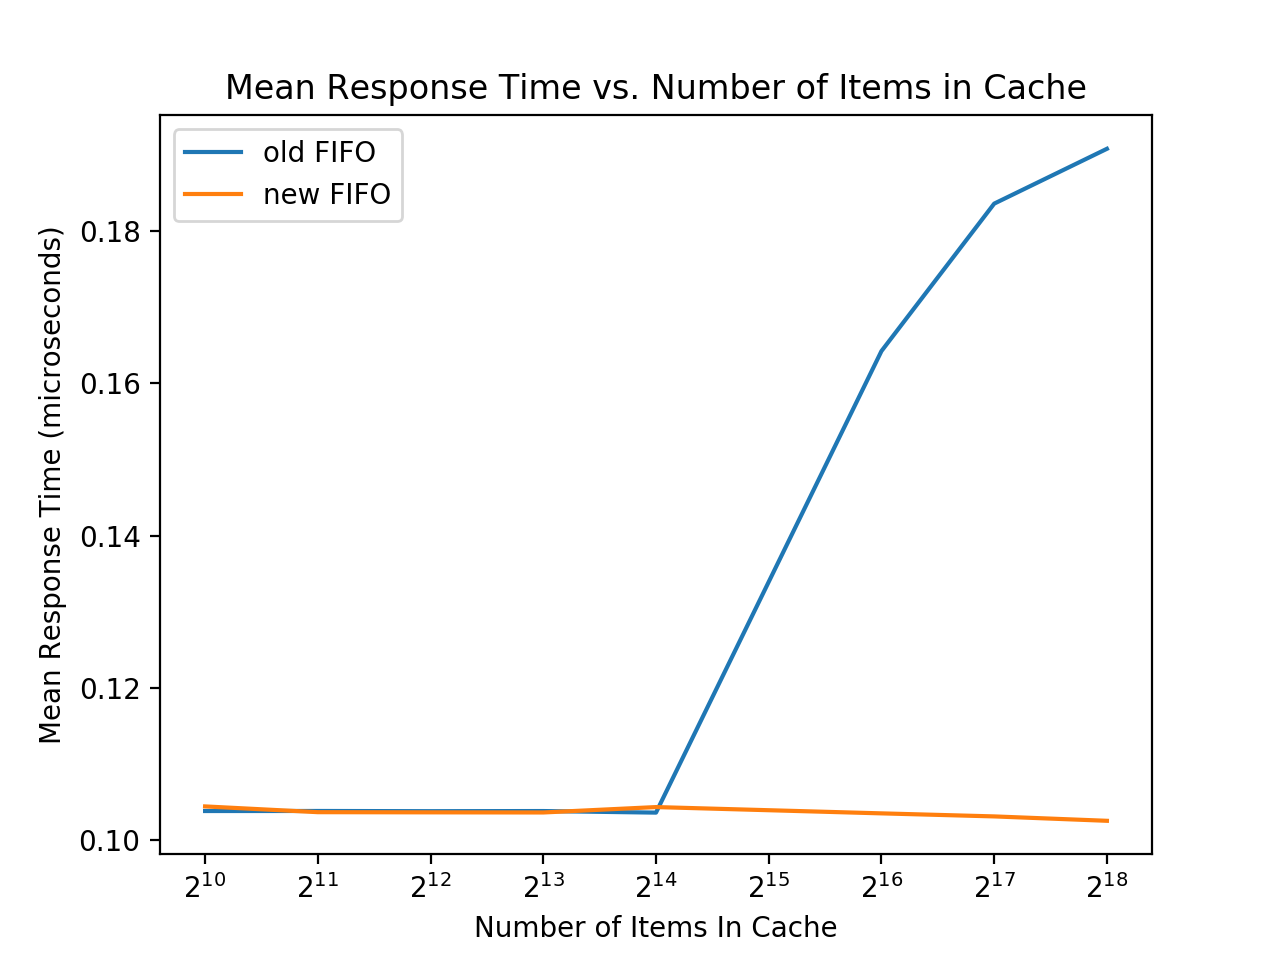
\includegraphics[scale=0.75]{resp_time_items_cache_newold.png}
\end{center}



\end{document}